\documentclass{article}
\usepackage{graphicx}
\usepackage{amsmath}
\usepackage{slashed}
\usepackage{tikz}
\usetikzlibrary{matrix}
\usepackage[a4paper, total={6in, 8in}]{geometry}

\begin{document}

\title{The Geometry of the Yang-Mill's Field}
\author{Christopher Milke}

\maketitle

\section{Introduction}
        The effort of this brief paper will be to derive the QED lagrangian (and to a lesser degree a general $SU(N)$) from a geometric perspective. We start, as usual, by defining the pure fermion field as the spin-one-half solutions to the Dirac Equation, and construct our lagrangian density as:

        $ \mathcal{L} =  i \bar{\Psi} \slashed\partial_\mu \Psi - m \bar{\Psi} \Psi   $

        From here, the usual next step is to demand invariance of the Lagrangian under local $U(1)$ (Gauge) tranformations. $U(1)$ gauge tranformations take the form: 

        $ \Psi(x) \rightarrow e^{-i \theta(x)} \Psi(x) $ and $ \bar\Psi(x) \rightarrow e^{+i \alpha(x)} \bar\Psi(x) $

        As the partial derivative of $\Psi$ does not transform this way in the lagrangian density, we introduce a new term into the lagrangian, 
        $  \bar{\Psi} \gamma^\mu \Psi A_\mu(x) $, which cancels the non-gauge-invariant part of the derivative. The new term with $A_\mu(x)$ can then be lumped in with the derivative term, to create a so-called ``Covariant'' derivative,
        $ D_\mu \equiv \partial_\mu - i e A_\mu $

        This is where I wish to diverge a bit. Instead of constructing the gauge field on the premise of gauge invariance, I will construct it on the basis of parallel transporting the fermion field through an internal $U(1)$ space.


\section{The $U(1)$ Vector Fermion Field}
        We begin our discussion of the gauge field with a look at the fermion field $\Psi(x)$. We can, naively (i.e. ignoring gauge symmetry), define the fermion field as: 
        $\Psi \equiv \mathbf{S}(x)$, with $\mathbf{S}(x)$ the four component spinor of the fermion. This is a vector in space-time, but we want to extend it as a vector in 
        
        We introduced local $U(1)$ transformations in the introduction, but this time around we will not be introducing $U(1)$ as a mere symmetry demand. Instead, we introduce local phase as a geometric space our fermion must traverse in the same manner as coordinate space-time. First let us define an accurate depiction of the fermion field:
        $\Psi \equiv \mathbf{S}(x) \cdot e^{i \phi(x)}$

        The obvious difference now is of course the coordinate-dependent complex phase. This is only one way to view the phase however. In pursuit of a more geometrically sound interpretation, we can expand the complex exponential into a real and imaginary component. Furthermore, the real and and imaginary components can be imagined not as complex components, but rather as components of an internal two-dimensional vector space. Labelling the two internal dimensions as $\alpha_1$ and $\alpha_2$, the fermion field takes the form:
        $\Psi =  \mathbf{S}(x) \left[ \alpha_1(x) \hat\alpha_1 + \alpha_2(x) \hat\alpha_2 \right]$ 

        The fermion field now acts like a vector field not only in space-time, but also in $U(1)$ space, with $\alpha_1$ and $\alpha_2$ providing the components of direction of the $U(1)$ vector, and $\mathbf{S}$ providing the vector in four-dimensional space-time. As such, we can finally take a sensible look at the covariant derivative, in the context of parallel transport.


\section{Parallel Transport}
        Conceptually, parallel transport is just another way of taking vector derivatives. In general relativity, this kind of differentiation is of crucial importance, and is mathematically very challenging. Here though, with our internal two-dimensional space, parallel transport is fairly simple. Typically, vector calculus involves performing derivatives on each component of the vector seperately. As one moves across the vector space, the components of the vector change independently of each other, and so the derivatives (be it a divergence, curl, or otherwise) track the rate of change of the components independent of one another. Parallel transport takes a slightly different approach. In parallel transport, the idea is that not only is the vector changing, but so is the \textit{geometry} which the vector traverses. In this case, it is not enough to only look at the changes in the vector components, because a change in the vector component from one point in the geometry to the next is the sum of two seperate changes: the true change of the vector, and the change of the geometry itself. A covarient derivative then, is a derivative meant to seperate these changes, and present only the true change of the vector, correcting for the changes in geometry.

        With the description of covariant derivatives out of the way, we turn to the trivial case of the covariant derivative of our fermion vector field. Seeking to replicate the method of parallel transport we seperate the fermion vector into true changes and geometric changes. I claim it as trivial because, in our formulation of QED, we find that the only part of the fermion vector which is not a result of geometric changes is the Spinor Amplitude. All of the $U(1)$ vector components of $\Psi$ we then attribute purely to changes in the internal $U(1)$ geometry. An appropriate covariant derivative will then exclusively compare changes in the magnitude of the fermion field, and exclude all changes in the phase. As the fermion field is merely a product of the spinor and phase, the covarient derivative then amounts to nothing more than canceling out part of the product rule:
        We define the covariant derivative as $ D_\mu \equiv \partial_\mu + \Gamma_\mu $, with $\Gamma_\mu$ being the connection coefficient,
        and demand that the covariant derivative of $ \Psi(x) $ take the derivative of only $\mathbf{S}(x)$, so that
        $D_\mu \Psi(x) = [ \partial_\mu \mathbf{S}(x) ] \cdot e^{i\phi(x)} $ . Then
        
        $ (\partial_\mu + \Gamma_\mu) [ \mathbf{S}(x) \cdot e^{i\phi(x)} ] $ 
        $ = (\partial_\mu \mathbf{S}(x) ) \cdot e^{i\phi(x)} +
             \mathbf{S}(x)  \cdot (\partial_\mu e^{i\phi(x)}) +
             \mathbf{S}(x)  \cdot e^{i\phi(x)} \Gamma_\mu $

        The unwanted term, the partial of the phase factor, is the only term that needs to be cancelled by the $\Gamma_\mu$. Thus the connection coefficient term here is simply $ -  \mathbf{S}(x)  (\partial_\mu e^{i\phi(x)})  $, which means 
        $\Gamma_\mu = - i \partial_\mu \phi(x) $. Pulling out a factor of $e$, we can relate the connection coefficient to the gauge field
        as $A_\mu \equiv \frac{1}{e} \partial_\mu \phi(x)$ returning us to the form of the covariant derivative we found in the introduction,
        $ D_\mu \equiv \partial_\mu - i e A_\mu $.


\section{Translations and the Field Tensor}
        Having derived the covarient derivative, we turn to a profound effect gauge invariance has on our lagrangian, in the form of translation. What we will find is that translation is no longer a trivial operation, and ultimately gives the connection coefficient $A_\mu$ a life of its own in the form of the electromagnetc field tensor. First, let's start with simply translating a fermion field.
        
        A translation over some displacement vector $\Delta x^\mu$ can in general be represented using the generator of translations,
        $e^{-i \Delta x^\mu \hat p_\mu}$ = $e^{- \Delta x^\mu \partial_\mu}$. We can immediately see the problem with this though. The translation operator contains a derivative, which we already know will render our translated lagrangian gauge-variant. This effectively means our lagrangian is no longer invariant under translations, which we know is wrong. The solution to this issue is to do exactly what we did before: replace the derivative with a covariant derivative:
        $e^{- \Delta x^\mu \partial_\mu} \rightarrow e^{- \Delta x^\mu D_\mu}$.
        Physically, exchanging the derivative for a covariant derivative corresponds to the fact that when we translate our field, we must also translate our gauge. In some sense, we really need two translation operators; one for the field
        $e^{-i \Delta x^\mu \hat p_\mu}$, and the other for the local phase
        $e^{-i \Delta x^\mu (-e A_\mu)}$. As both operators are complex exponentials, they combine as 
        $e^{-i \Delta x^\mu [( -i \partial_\mu) + (-e A_\mu)]} = e^{ - \Delta x^\mu D_\mu }$. As a side note, this suggests an interesting interpretation of the quantity $( -e A_\mu )$ as the momentum of the local phase.

        With our translation operator in hand, we can now construct the electromagnetic field tensor. To do this, we will translate a fermion field in a closed loop, with four successive, orthogonal, infinitesimal translations in two dimesions. Physically, this can be thought of as moving a fermion a tiny distance east, then north, then west, then back south to where it started. Mathematically, this means operating on a fermion field with four seperate translation operators:
        $ \Psi'(x) = T_{DA} T_{CD} T_{BC} T_{AB} \Psi(x) $

        \vspace{5pt}
        \begin{center} 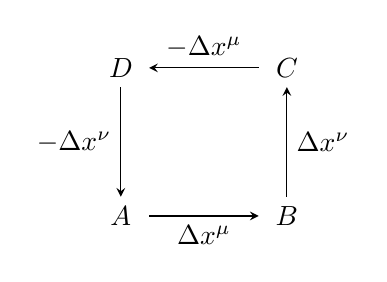
\begin{tikzpicture}
                \matrix (m) 
                [matrix of math nodes,row sep=4em,column sep=4em,minimum width=2em] {
                        D & C \\
                        A  & B \\ 
                }; 
                \path[-stealth] 
                        (m-2-1) edge node [below] {$\Delta x^\mu$} (m-2-2) 
                        (m-2-2) edge node [right] {$\Delta x^\nu$} (m-1-2)
                        (m-1-2) edge node [above] {$-\Delta x^\mu$} (m-1-1)
                        (m-1-1) edge node [left] {$-\Delta x^\nu$} (m-2-1);
        \end{tikzpicture} \end{center}
        \vspace{5pt}
        
        
        Over an infinitesimal displacement, we can expand the translation exponential out to first order in the displacement,
        $ T \approx 1 - \Delta x^\mu D_\mu $, and then our translated field is:


        $ \Psi'(x) = (1 + \Delta x^\nu D_\nu)(1 + \Delta x^\mu D_\mu)(1 - \Delta x^\nu D_\nu)(1 - \Delta x^\mu D_\mu) \Psi(x) $

        $ = (1 + \Delta x^\nu D_\nu + \Delta x^\mu D_\mu + \Delta x^\nu \Delta x^\mu D_\nu D_\mu)
        (1 - \Delta x^\nu D_\nu - \Delta x^\mu D_\mu + \Delta x^\nu \Delta x^\mu D_\nu D_\mu) \Psi(x) $

        \vspace{5pt}

        Disregarding second order terms in the displacment vector:

                $ = (1 + \Delta x^\nu D_\nu + \Delta x^\mu D_\mu + \Delta x^\nu \Delta x^\mu D_\nu D_\mu $

        \hspace{20pt}$ - \Delta x^\nu D_\nu - \Delta x^\mu D_\mu + \Delta x^\nu \Delta x^\mu D_\nu D_\mu $

        \hspace{20pt}$ - \Delta x^\nu \Delta x^\mu D_\nu D_\mu - \Delta x^\mu \Delta x^\nu D_\mu D_\nu) \Psi(x) $

        \vspace{5pt}

        $ = (1 + \Delta x^\nu \Delta x^\mu D_\nu D_\mu - \Delta x^\mu \Delta x^\nu D_\mu D_\nu) \Psi(x)$

        $ = \left(1 + \Delta x^\mu \Delta x^\nu ( D_\nu D_\mu - D_\mu D_\nu) \right) \Psi(x)$, quickly renaming indices:

        $ = \left(1 + \Delta x^\nu \Delta x^\mu ( D_\mu D_\nu - D_\nu D_\mu) \right) \Psi(x)$

        $ = \left(1 + \Delta x^\mu \Delta x^\nu [ D_\mu , D_\nu ] \right) \Psi(x)$.

        \vspace{5pt}
        Finally, identifying the commutator of the covariant derivatives as
        $ [ D_\mu , D_\nu ] = - i g F_{\mu \nu} $, and the area of the box we went around as
        $ R^{\mu \nu} = \Delta x^\mu \Delta x^\nu $, we arrive at:

        $ \Psi'(x) = \left(1 -i g R^{\mu \nu} F_{\mu \nu} \right) \Psi(x)$

        What this final result demonstrates is that our fermion field cannot be translated in a closed loop without generating an extra term proportianal to $F_{\mu \nu}$. The consequence of this is that we must introduce an additional term to our lagrangian,
        $-\frac{1}{4}F_{\mu \nu} F^{\mu \nu}$, as a correction. This new term however, behaves as a massless propagator of the connection coefficient $A_\mu$, indicating that $A_\mu$ is in fact a particle field of its own. Experimentally, we already know this is the case, and so we recognize $A_\mu$ as the field associated with the photon, and $F^{\mu \nu}$ as the electromagnetic field tensor.






        




        \clearpage
        \section{Sources}
                \begin{itemize}
                        \item \underline{Quantum Field Theory}; \textit{Lewis H. Ryder}; 1985
                        \item \underline{Introduction to Quantum Field Theory}; \textit{Michael E. Peskin, Daniel V. Schroeder}; 1951
                        \item \underline{Quantum Field Theory}; \textit{Mark Srednecki}; 2007
                        \item \underline{Relativity, Gravitation and Cosmology 2E}; \textit{Ta-Pei Cheng}; 2010
                \end{itemize}


\end{document}
